\section{Introduction}
\label{sec:intro}

An assistant that talks with the same person for months accumulates more history than it can reread at every turn.
Rereading everything grows more expensive with every conversation and stops being possible once the history outgrows the context window.
Long-term memory systems therefore decide which parts of the history the assistant sees, and most of them decide it when the history is written: Mem0 extracts and updates facts~\citep{chhikara2025mem0}, Zep builds a temporal knowledge graph~\citep{rasmussen2025zep}, and MemOS, EverMemOS, Nemori and MIRIX organize conversations into memory units, episodes or typed stores~\citep{li2025memos,evermemos2026,nan2025nemori,wang2025mirix}.

\paragraph{The cost of writing first.}
Rewriting a conversation when it is stored pays for understanding before the question is known.
Every message is processed whether or not it is ever asked about, and what the extractor drops or distorts cannot be recovered when a question finally reveals what mattered.
It also moves judgment away from the moment with the most information for it: the question, the recent dialogue and the candidate records are known together only when the question is asked.

\paragraph{Remembering fast and slow.}
Dual-process accounts of thinking separate a fast, automatic System~1 from a slow, deliberate System~2~\citep{kahneman2011thinking}.
We observe that the work of memory divides the same way.
Most of it is System~1 work: small, independent yes/no questions with explicit criteria, such as whether the reply should use this record, whether a later message has made it obsolete, or whether it gives the second of the two dates the question needs.
System One models such as \jev{} answer such questions by the dozen in a third of a second~\citep{jev2026}.
Only a little is System~2 work: wording a few searches, naming the facts the reply needs, and computing the answer from what is shown, which an LLM does well but slowly.
Because the judging is fast, \sys{} can read raw, dated records when a question arrives instead of rewriting them in advance: an LLM plans (System~2), \jev{} judges (System~1), and rules with explicit budgets decide what to page, rewrite and show.
Slow work that no reply can wait for runs in the background: for evidence that no question points to, such as an instruction given once, every mention of a topic or a value that changed, \sys{} consolidates each record once into an index of topic timelines, value histories and standing instructions that links back to the records.
The index directs reading, and the records remain the evidence.

\paragraph{Our contributions.}
\sys{} runs as a second instance of an open-source agent harness~\citep{dsh2026} and hands the unchanged main agent one View per turn.
Our contributions are:
\begin{itemize}
  \item \textbf{Memory as System~1 and System~2} (\cref{sec:design,sec:impl}): a memory agent that gives judging to a decision model and planning and answering to an LLM, over raw records and a consolidated index that points back to them, with ordinal rules under explicit budgets; it is built entirely from the harness's plugins.
  \item \textbf{Accuracy at small context} (\cref{sec:main}): under the protocol of OmniMemEval, a public re-evaluation of 14 memory systems with gpt-4.1-mini answering~\citep{omnimemeval2026}, \sys{} is the most accurate system on LoCoMo (\finLoCoMo\%) and second on \lme{} (\finLME\%), from under 4k tokens of context per question, with the lowest effective cost index on LoCoMo.
  \item \textbf{Stronger readers, bounded cost} (\cref{sec:reasoning,sec:scale}): with a reasoning reader, \sys{} reaches \dsFinLoCoMo\% on LoCoMo and \dsFinLME\% on \lme, level on \lme{} with the best published results; from BEAM's 100K tier to its 10M tier, with 80 times as many records, its cost per question grows by a factor of \beamTenCostRatioC.
  \item \textbf{Judging belongs to System~1} (\cref{sec:system1}): on the same records, \jev{} separates gold evidence better than two LLM judges (AUC 0.942 against 0.900 and 0.853) at 3--11 times lower latency.
\end{itemize}
\Cref{fig:tradeoff} summarizes the comparison on the two most widely reported benchmarks: \sys{} is the only system above 80\% on both that sends the answering model fewer than 4k tokens per question.

\begin{figure}[t]
\centering
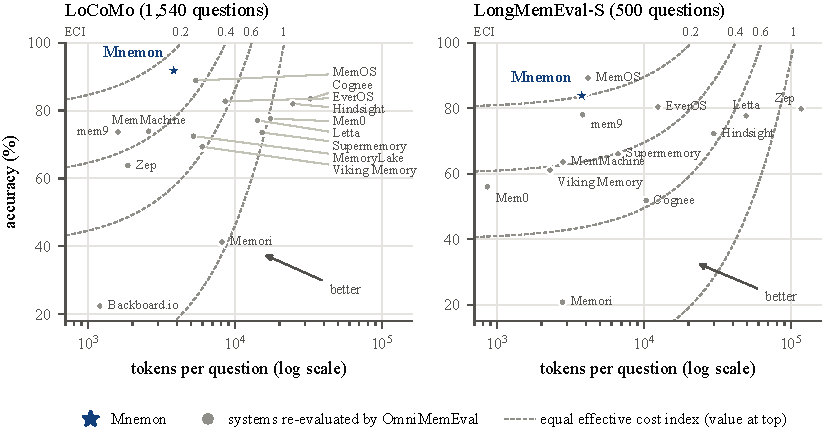
\includegraphics[width=\linewidth]{figures/tradeoff.pdf}
\caption{Accuracy against context per question for \sys{} (star) and the 14 systems re-evaluated by OmniMemEval, all with gpt-4.1-mini answering. Dashed lines join points of equal effective cost index (\cref{sec:setting}); up and to the left is better.}
\label{fig:tradeoff}
\end{figure}
